\newpage
\clearpage
\section{Results and Outlook}
    This is the $p_T$ spectrum of the yield for $\omega$ and $\phi$. Since the cross section has not been calculated for the vertical axis yet, a comparison with other experimental results cannot be made. However, a distribution with an exponential dependence on $p_T$ can be observed.
    \begin{figure}[htbp]
        \centering
        % Left side figure
        \begin{minipage}{0.45\textwidth} % Specify width using minipage
            \centering
            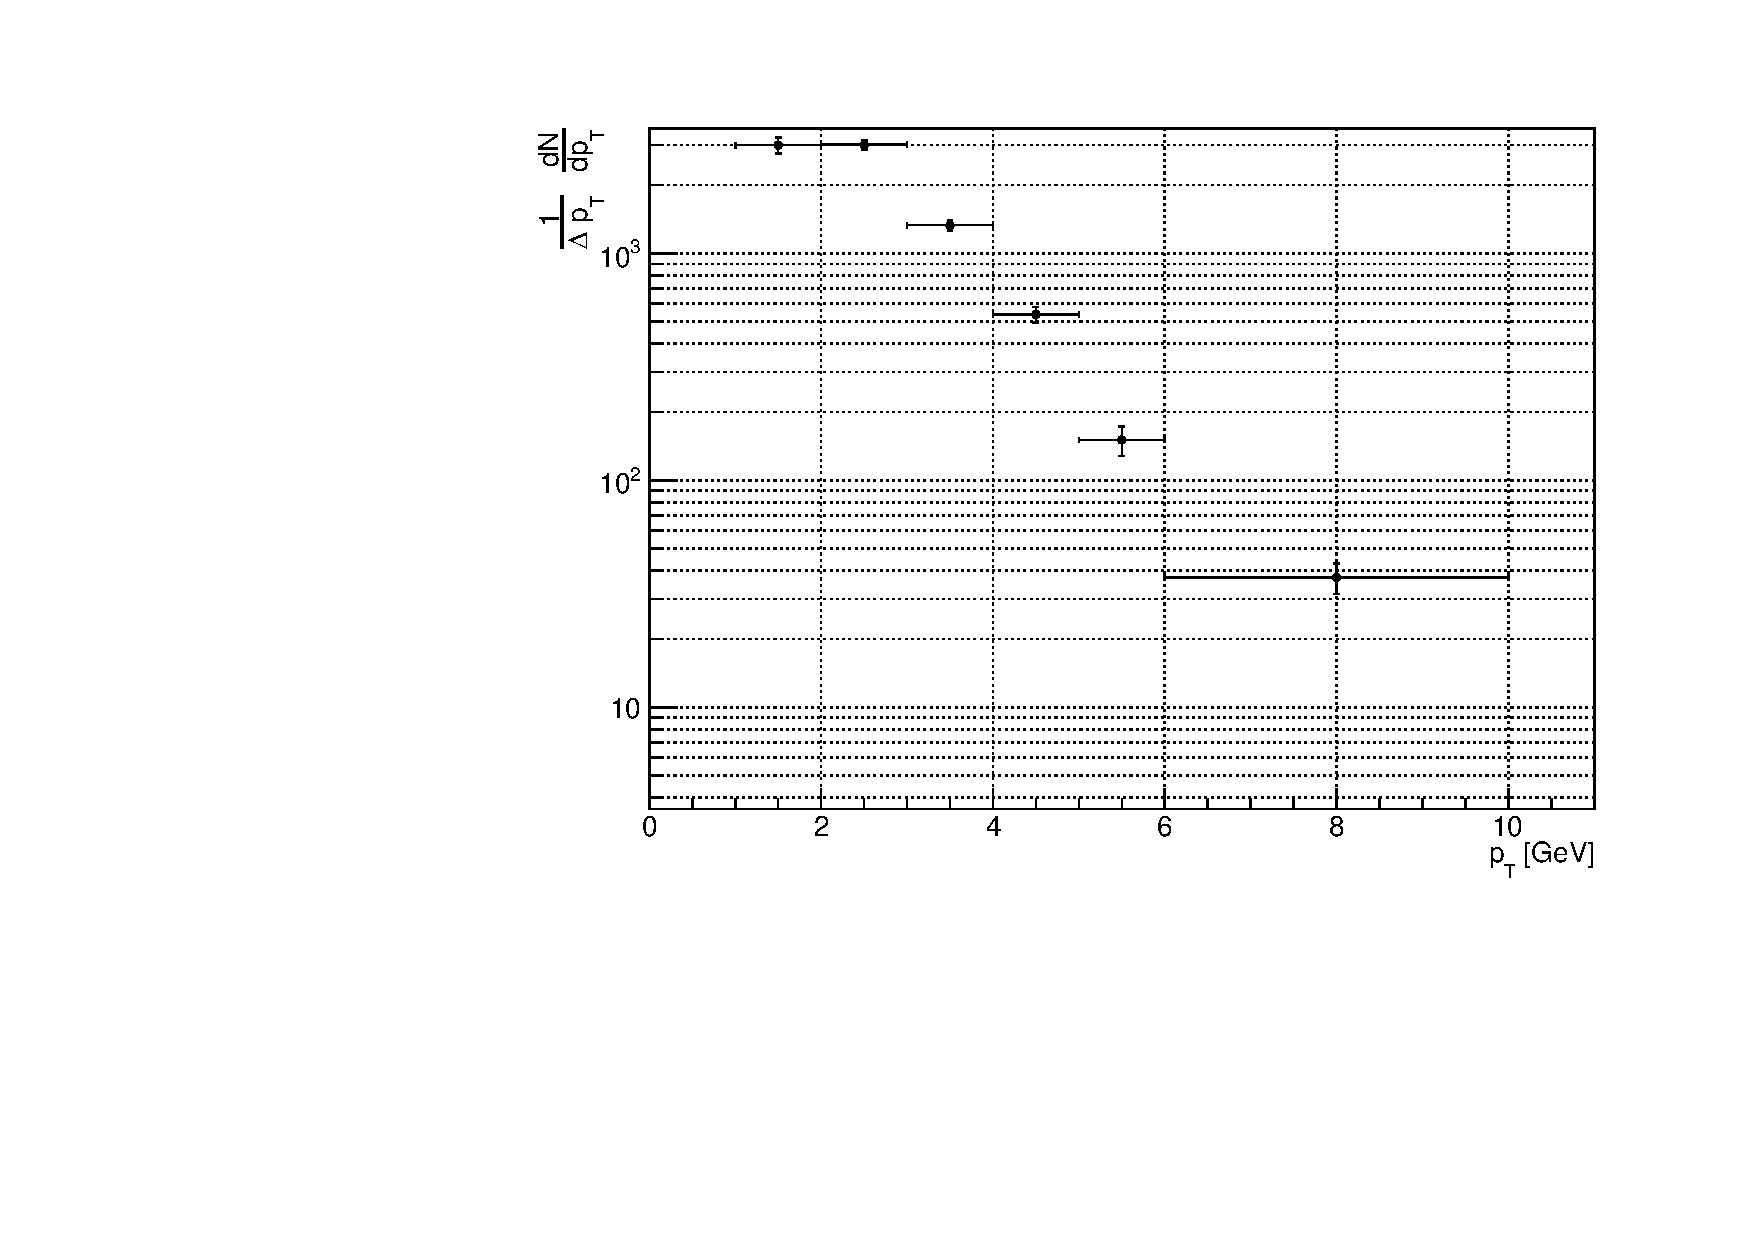
\includegraphics[width=\textwidth]{fig/4_omega_yield.pdf} % Left side image
            \caption{$\omega$ yield}
            \label{fig:omega_yield}
        \end{minipage}
        % Right side figure
        \hfill
        \begin{minipage}{0.45\textwidth}
            \centering
            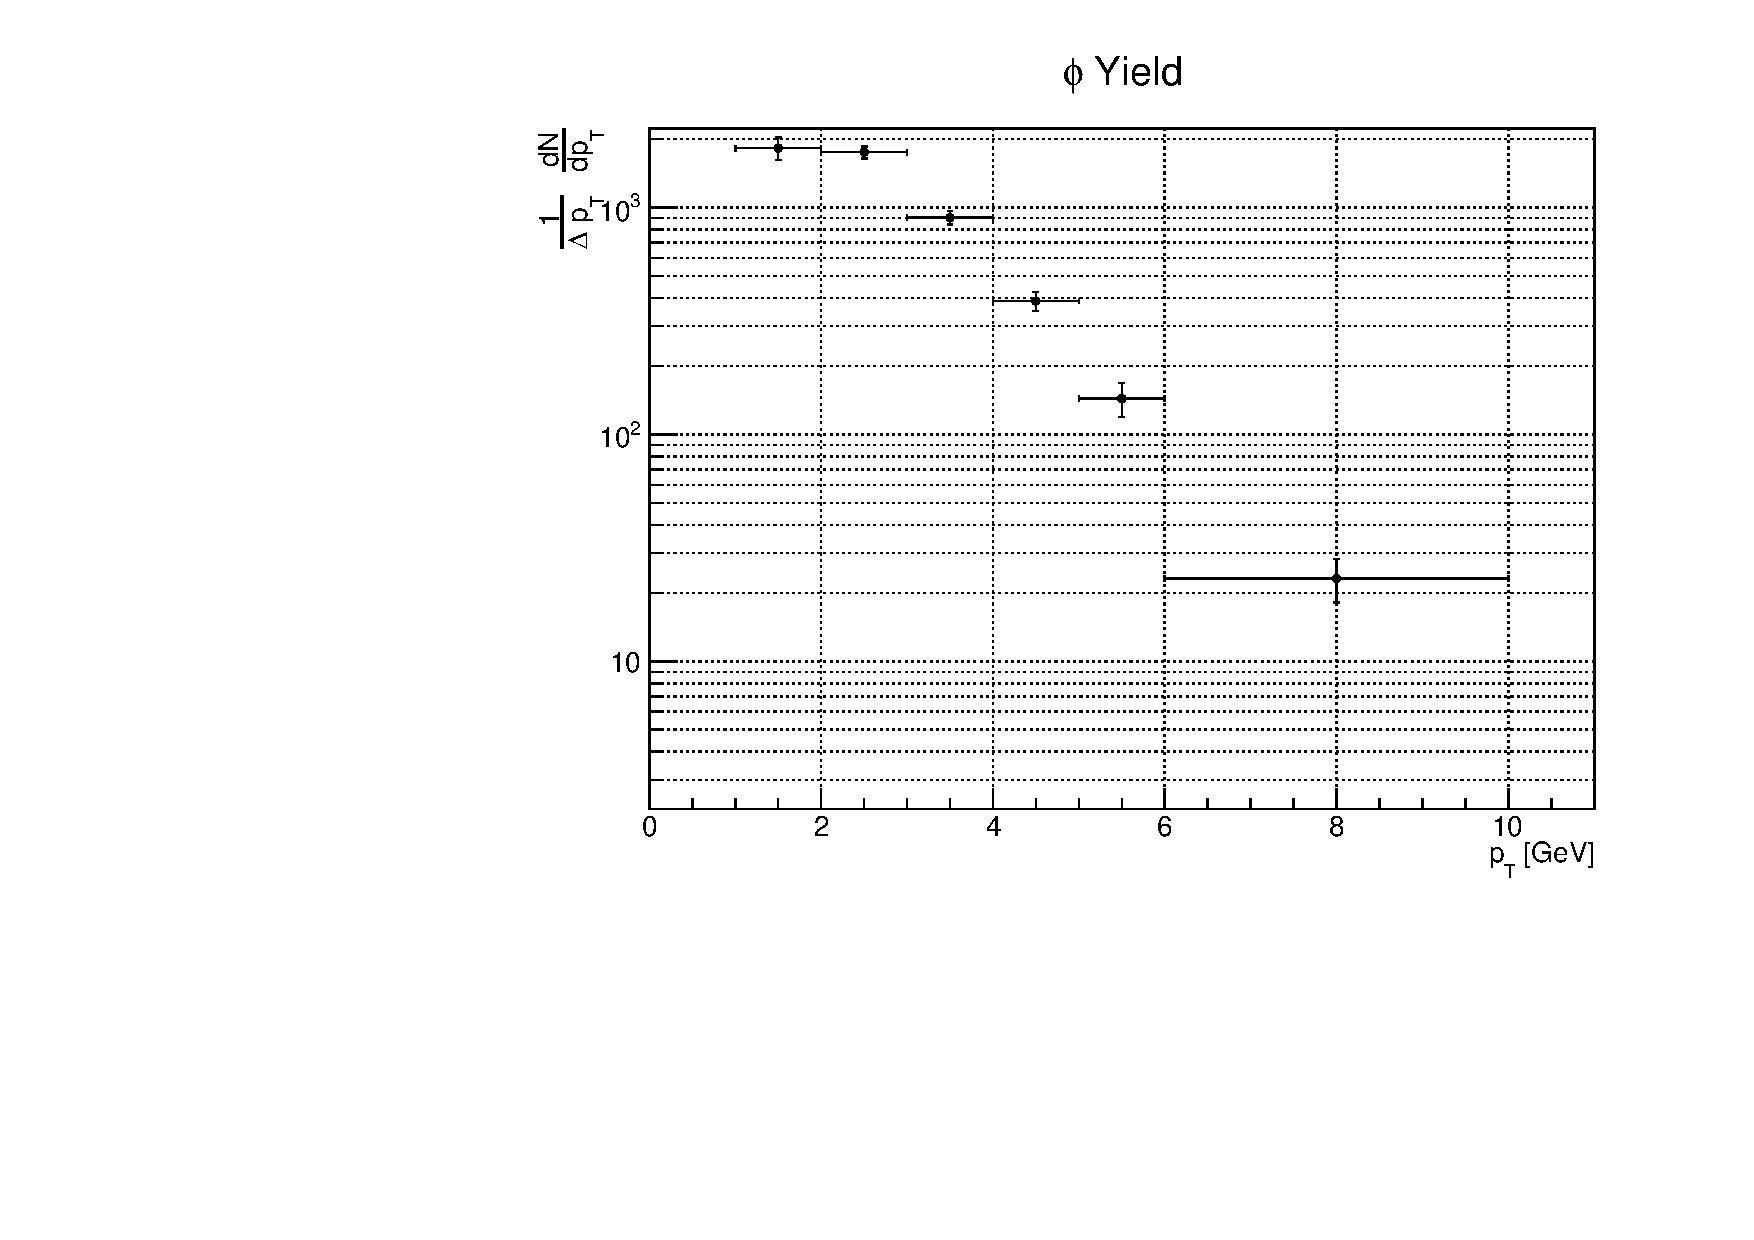
\includegraphics[width=\textwidth]{fig/4_phi_yield.pdf} % Right side image
            \caption{$\phi$ yield}
            \label{fig:phi_yield}
        \end{minipage}
    \end{figure}
    As for future prospects, simulations of $\omega \rightarrow \mu\mu$ and $\phi \rightarrow \mu\mu$ will be conducted, followed by acceptance $\times$ efficiency corrections. The goal is to determine the production cross-section for $\omega$ and $\phi$ in forward muon pairs.
